\documentclass[12pt]{article}
\usepackage{amsmath}
\usepackage{times}
\usepackage{graphicx}
\usepackage[left=1.5in,right=1.0in,top=1.0in,bottom=1.0in]{geometry}
\newcommand{\nd}{\noindent}
\newcommand{\mainsize}{\fontsize{16pt}{12pt}\selectfont}
\newcommand{\msize}{\fontsize{14pt}{12pt}\selectfont}
\begin{document}
\large  
\parskip 3mm 
\title{\textbf{Traffic Prediction for Intelligent Transportation System using Machine Learning}}
\author{}
\date{}
\maketitle
\tableofcontents
\newpage
\section{\mainsize{\textbf{LITERATURE SURVEY}}}
Many works has already been proposed for predicting traffic using intelligent machine learning systems like Fei-Yue Wang proposed parallel control and management for intelligent transportation systems and Chun-Hsin Wu, Jan-Ming Ho, and D. T. Lee proposed deployment of support vector regression for mapping traffic densities, Jason Brownlee has proposed the deployment of bagging and random forest ensemble models for traffic predicitons. 

\nd But many of these models use shallow traffic models and are still somewhat failing due to the enormous dataset dimension. 
This is where our project comes in clutch 

\subsection{\msize{\textbf{\textbf{METHODS USED IN RESEARCH PAPERS}}}}
Some of the various types of research techniques which has been deployed are
\subsubsection{\textbf{TRANSACTIONS ON INTELLIGENT TRANSPORT }}
$\text{Fei-Yue Wang et al}^{[1]}$ :The development and deployment of Intelligent Transportation System  provide better accuracy for Traffic flow prediction. It is deal with as a crucial element for the success of advanced traffic management systems, advanced public transportation systems, and traveller information systems. 

\subsubsection{\textbf{ ACCELERATED INCIDENT DETECTION VIA VEHICLE KINEMATICS}}
$\text{Yongchang Ma, Mashrur Chowdhury, Mansoureh Jeihani, and Ryan Fries}^{[2]}$ proposed The dependency of traffic flow is dependent on real-time traffic and historical data collected from various sensor sources, including inductive loops, radars, cameras, mobile Global Positioning System, crowd sourcing, social media. Traffic data is exploding due to the vast use of traditional sensors and new technologies, and we have entered the era of a large volume of data transportation. Transportation control and management are now becoming more data-driven.

\subsubsection{\textbf{DELEGATE MULTI AGRENT SYSTEM}}
$\text{Rutger Claes, Tom Holvoet, and Danny Weyns}^{[3]}$ have proposed the use of decentralized approach for anticipatory vehicle routing using delegate multiagent systems. This helps in advanced detection of high density traffic flows at various junctures 

\subsubsection{\textbf{SEMANTIC INDEXING}}
$\text{MehulMahrishiandSudhaMorwal}^{[4]}$ proposed the use of multi-layer concepts of neural networks to mining the inherent properties in data from the lowest level to the highest level 

\subsubsection{\textbf{SHORT RANGE COMMUNICATION}}
$\text{Joseph D Crabtree and Nikiforos Stamatiadis}^{[5]}$ proposed the implementation via driver as-sistance system (DAS), autonomous vehicles (AV)and Traffic Sign Recognition (TSR)

\subsubsection{\textbf{KINEMATIC DATA FROM PROBE VEHICLES}}
$\text{H Qi, RL Cheu, and DH Lee.}^{[6]}$ proposed the use of probe vehicles to gather test and simulation data to better understand the nature of the traffic 

\subsubsection{\textbf{LONG SHORT TERM MEMORY NETWORKS}}
$\text{Z. Zhao, W. Chen, X. Wu, P. C. Y. Chen, and J. Liu.}^{[7]}$ proposed the implementation of LONG SHORT TERM NEURAL NETS. In this control, strategies identify the potential congestions on the roads, and it directed to the passengers to take some alternative routes to their destinations. 

\subsubsection{\textbf{DEEP LEARNING IN NETWORKING}}
$\text{C. Zhang, P. Patras, and H. Haddadi.}^{[8]}$ proposed the idea of deploying deep neural nets in mobile and wireless communications. In DL, use concepts of a neural network, by using this feature, it is beneficial to find network dynamics (such as spectrum availability, congestion points, hotspots, traffic bottleneck. 

\subsubsection{\textbf{TRAVEL TIME PREDICTION}}
$\text{Chun-Hsin Wu, Jan-Ming Ho, and D. T. Lee.}^{[9]}$ proposed studying the travel time via support vector regression. Support Vector Regression (SVR) tries to fit as many instances as possible on the road while limiting margin violations. 

\subsubsection{\textbf{DECISION TREE METHODS}}
$\text{Yan-Yan Song and LU Ying.}^{[10]}$proposed deploying decision trees to study the traffic. Decision Trees identify its results by performing a set of tests on the training dataset

\subsubsection{\textbf{MERGING MOBILITY AND ENERGY}}
$\text{Yiming He, Mashrur Chowdhury, Yongchang Ma, and Pierluigi Pisu.}^{[11]}$ proposed merging of mobility and energy visions which were in conflict with one another via SVM. The SVM is beneficial for high dimensional spaces, and it also helps in the condition where a number of samples are less than the number of dimensions

\subsubsection{\textbf{BAGGING AND RANDOM FOREST}}
$\text{Jason Brownlee}^{[12]}$proposed deploying bagging and random forest models. The random forest algorithm is a robust machine learning algorithm. It is defined as bootstrap aggregation. The random forest algorithm is based on forecasting models, and it is mostly used to classify the data. The bootstrap algorithm is used to generate multiple models from a single training data sets. A bootstrap algorithm has also used a sample to estimate statistical quantities.
\newpage 
%%%%%%%%%%%%%%%%%%%%%%%
\section{\mainsize{\textbf{DESIGN}}}
We have deployed some specific types of neural networks to predict and intelligently determine traffic density and congestion at various places. We have specifically chosen Deep Neural Networks because they can deal with high amounts of datasets and their enormous dimensions. The more the dimensions and dense the data is the better the performance of the model. This makes our model redundant to specific anomalies in the dataset. 

\nd If a small dataset has anomalies it will result in very biased models. But in high dimension datasets, the anomalies can be encoded or even discarded while having minuscule to no impact on the accuracy, because of the model moving on to another dimension without any anomalies 

\nd The types of Neural networks we have deployed for our model are : 

\nd 1. Long Short Term Memory Network 

\nd 2. Recurrent And Sequential Networks 

\nd 3. Dense Networks 

\nd 4. Feature Engineering- Generating Lag Features 

\nd 5. Rectified Linear Activation Function And Adam Optimiser 

\newpage 
\subsection{\msize{\textbf{\textbf{LONG SHORT TERM MEMORY NETWORKS}}}}
Long Short-Term Memory (LSTM) networks are a type of recurrent neural network capable of learning order dependence in sequence prediction problems. This is a behavior required in complex problem domains like machine translation, speech recognition, and more.

\nd LSTMs are a complex area of deep learning. It can be hard to get your hands around what LSTMs are, and how terms like bidirectional and sequence-to-sequence relate to the field. Recurrent neural networks are different from traditional feed-forward neural networks. This difference in the addition of complexity comes with the promise of new behaviors that the traditional methods cannot achieve.

\nd Recurrent networks have an internal state that can represent context information. They keep information about past inputs for an amount of time that is not fixed a priori, but rather depends on its weights and on the input data.

\nd A recurrent network whose inputs are not fixed but rather constitute an input sequence can be used to transform an input sequence into an output sequence while taking into account contextual information in a flexible way.

\nd The three basic requirements of recurrent neural networks are 

\nd 1. The system be able to store information for an arbitrary duration.

\nd 2. The system be resistant to noise i.e. fluctuations of the inputs that are random or irrelevant to predicting a correct output

\nd 3. That the system parameters be trainable 

\nd The standard RNNs fail to learn in the presence of time lags greater than 5 – 10 discrete time steps between relevant input events and target signals. The vanishing error problem casts doubt on whether standard RNNs can indeed exhibit significant practical advantages over time window-based feedforward networks. A recent model, “Long Short-Term Memory” (LSTM), is not affected by this problem. LSTM can learn to bridge minimal time lags in excess of 1000 discrete time steps by enforcing constant error flow through “constant error carrousels” (CECs) within special units, called cells

\begin{center}
\centerline{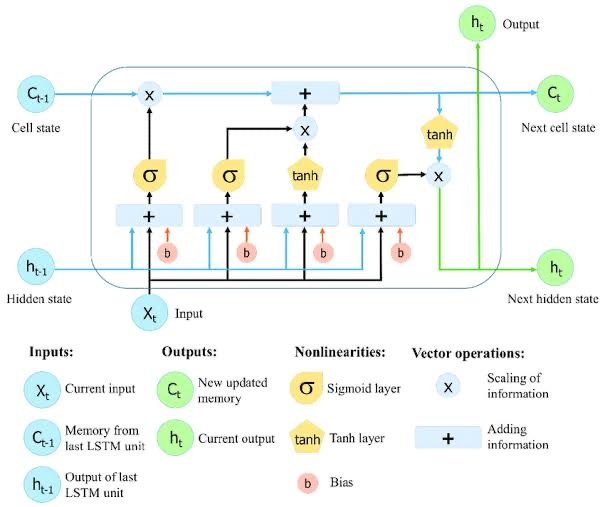
\includegraphics[scale=.5]{lstm.jpg}}
\end{center}

\nd Each memory cell’s internal architecture guarantees constant error ow within its constant error carrousel CEC… This represents the basis for bridging very long time lags. Two gate units learn to open and close access to error ow within each memory cell’s CEC. The multiplicative input gate affords protection of the CEC from perturbation by irrelevant inputs. Likewise, the multiplicative output gate protects other units from perturbation by currently irrelevant memory contents.

\nd The functions and equations driving an LSTM are : 

\begin{equation*}
i_t =\delta(x_t u^i + h_{t-1} W^i)
\end{equation*}

\begin{equation*}
f_t = \delta(x_t U^t + h_{t-1} W^t)
\end{equation*}

\begin{equation*}
o_t = \delta(x_t U^o + h_{t-1} W^o)
\end{equation*}

\begin{equation*}
C^{'}_t = \tanh(x_t U^i + h_{t-1} W^g)
\end{equation*}

\begin{equation*}
C_t = \delta(f_t C_{t-1} + i_t *  C^{'}_t)
\end{equation*}

\begin{equation*}
h_t = \tanh(C_t ) + o_t
\end{equation*}

\nd The functioning of LSTM can be visualized by understanding the functioning of a news channel’s team covering a murder story. Now, a news story is built around facts, evidence and statements of many people. Whenever a new event occurs you take either of the three steps.

\nd Let’s say, we were assuming that the murder was done by ‘poisoning’ the victim, but the autopsy report that just came in said that the cause of death was ‘an impact on the head’. Being a part of this news team what do you do? You immediately forget the previous cause of death and all stories that were woven around this fact.

\nd What, if an entirely new suspect is introduced into the picture. A person who had grudges with the victim and could be the murderer? You input this information into your news feed, right?

\nd Now all these broken pieces of information cannot be served on mainstream media. So, after a certain time interval, you need to summarize this information and output the relevant things to your audience. Maybe in the form of “XYZ turns out to be the prime suspect.”.

\nd The advantages and applications of LSTM include 

\nd 1. Language modelling or text generation, that involves the computation of words when a sequence of words is fed as input. Language models can be operated at the character level, n-gram level, sentence level or even paragraph level.

\nd 2. Image processing, that involves performing analysis of a picture and concluding its result into a sentence. For this, it’s required to have a dataset comprising of a good amount of pictures with their corresponding descriptive captions. A model that has already been trained is used to predict features of images present in the dataset. This is photo data. The dataset is then processed in such a way that only the words that are most suggestive are present in it. This is text data. Using these two types of data, we try to fit the model. The work of the model is to generate a descriptive sentence for the picture one word at a time by taking input words that were predicted previously by the model and also the image.

\nd 3. Speech and Handwriting Recognition

\nd 4. Music generation which is quite similar to that of text generation where LSTMs predict musical notes instead of text by analyzing a combination of given notes fed as input.

\nd 5. Language Translation involves mapping a sequence in one language to a sequence in another language. Similar to image processing, a dataset, containing phrases and their translations, is first cleaned and only a part of it is used to train the model. An encoder-decoder LSTM model is used which first converts input sequence to its vector representation (encoding) and then outputs it to its translated version.

\nd The limitations and drawbacks of LSTM includes : 

\nd 1. LSTMs became popular because they could solve the problem of vanishing gradients. But it turns out, they fail to remove it completely. The problem lies in the fact that the data still has to move from cell to cell for its evaluation. Moreover, the cell has become quite complex now with the additional features (such as forget gates) being brought into the picture.

\nd 2. They require a lot of resources and time to get trained and become ready for real-world applications. In technical terms, they need high memory-bandwidth because of linear layers present in each cell which the system usually fails to provide for. Thus, hardware-wise, LSTMs become quite inefficient.

\nd 3. With the rise of data mining, developers are looking for a model that can remember past information for a longer time than LSTMs. The source of inspiration for such kind of model is the human habit of dividing a given piece of information into small parts for easy remembrance.

\nd 4. LSTMs are prone to overfitting and it is difficult to apply the dropout algorithm to curb this issue. Dropout is a regularization method where input and recurrent connections to LSTM units are probabilistically excluded from activation and weight updates while training a network.

\newpage 
\subsection{\msize{\textbf{\textbf{RECURRENT AND SEQUENTIAL NETWORKS}}}}
Sequential networks are the logic networks with memory. An example is a single input single output network that produces 1 iff three consecutive l’s appear in the inputs. Sequential networks are represented by state diagrams or state tables. Flip-flops are used for memory elements. A design of a sequential network is done as follows: First, minimize the number of states. Second, assign a binary code to each state. Third, allocate flip-flops. And, finally, realize the networks for flip-flops and outputs

\nd Sequence models are the machine learning models that input or output sequences of data. Sequential data includes text streams, audio clips, video clips, time-series data and etc. Recurrent Neural Networks (RNNs) is a popular algorithm used in sequence models.

\nd One form of Sequential Neural networks are Recurrent Neural networks. Recurrent Neural Network (RNN) is a Deep learning algorithm and it is a type of Artificial Neural Network architecture that is specialized for processing sequential data. RNNs are mostly used in the field of Natural Language Processing (NLP). RNN maintains internal memory, due to this they are very efficient for machine learning problems that involve sequential data. RNNs are also used in time series predictions as well.

\nd The main advantage of using RNNs instead of standard neural networks is that the features are not shared in standard neural networks. Weights are shared across time in RNN. RNNs can remember its previous inputs but Standard Neural Networks are not capable of remembering previous inputs. RNN takes historical information for computation. 

\begin{equation*}
L(y^{'} , y) = \sum_{t=1}^{T}{L(y^{'<t>},y^{<t>})}
\end{equation*}

\nd There are several RNN architectures based on the number of inputs and outputs 

\nd 1. One to Many Architecture: Image captioning is one good example of this architecture. In image captioning, it takes one image and then outputs a sequence of words. Here there is only one input but many outputs.

\nd 2. Many to One Architecture: Sentiment classification is one good example of this architecture. In sentiment classification, a given sentence is classified as positive or negative. In this case, the input is a sequence of words and output is a binary classification

\nd 3. Many to Many Architecture: There are two cases in many to many architectures

\begin{center}
\centerline{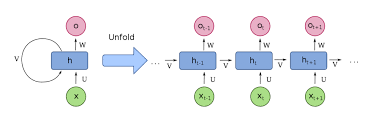
\includegraphics[scale=.5]{seq.png}}
\end{center}

\nd The advantages of Recurrent Neural Networks are : 

\nd 1. RNN can process inputs of any length.

\nd 2. An RNN model is modeled to remember each information throughout the time which is very helpful in any time series predictor.

\nd 3. Even if the input size is larger, the model size does not increase.

\nd 4. The weights can be shared across the time steps.

\nd 5. RNN can use their internal memory for processing the arbitrary series of inputs which is not the case with feedforward neural networks.

\nd The disadvantages of recurrent neural networks are 

\nd 1. Due to its recurrent nature, the computation is slow.

\nd 2. Training of RNN models can be difficult.

\nd 3. If we are using relu or tanh as activation functions, it becomes very difficult to process sequences that are very long.

\nd 4. Prone to problems such as exploding and gradient vanishing.

\newpage 
\subsection{\msize{\textbf{\textbf{DENSE NETWORKS}}}}
Dense layer is the regular deeply connected neural network layer. It is most common and frequently used layer. Dense layer does the below operation on the input and return the output.

\nd The “Deep” in deep-learning comes from the notion of increased complexity resulting by stacking several consecutive (hidden) non-linear layers. Here are some graphs of the most famous activation functions like Sigmoid, Relu, Hyperbolic tangent and many more 

\nd Obviously, we can see now that dense layers can be reduced back to linear layers if we use a linear activation

\nd Dense layers add an interesting non-linearity property, thus they can model any mathematical function. However, they are still limited in the sense that for the same input vector we get always the same output vector. They can’t detect repetition in time, or produce different answers on the same input

\begin{center}
\centerline{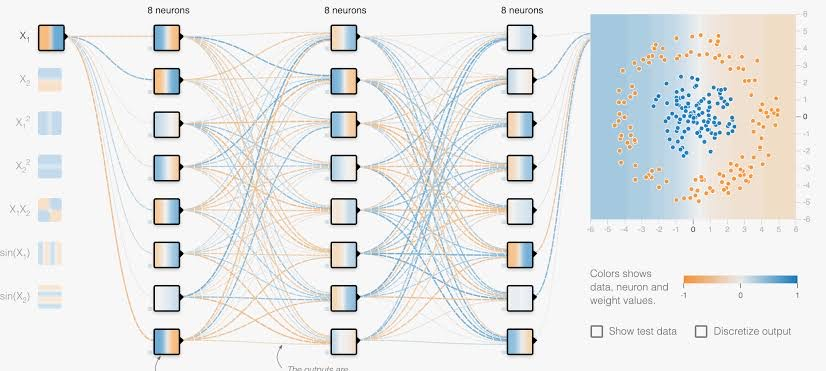
\includegraphics[scale=.5]{dense.jpg}}
\end{center}

\nd The output shape of the Dense layer will be affected by the number of neuron units specified in the Dense layer. For example, if the input shape is (8,) and number of unit is 16, then the output shape is (16,). All layer will have batch size as the first dimension and so, input shape will be represented by (None, 8) and the output shape as (None, 16). Currently, batch size is None as it is not set. Batch size is usually set during training phase.

\nd From an architecture point of view, any single convolution can be replaced by a Dense layer that would perform the same association of neighboring pixels for each pixel. It would mean one neuron per pixel with not-null coefficients only on the neighbors. Convolutional layer is enforcing parameter sharing: the processing of each pixel is identical by design, not by learning. It means a dramatic reduction in the number of parameters to learn, still with a very good performance, as we will see in the evaluation section.

\nd some of the activation functions are : 

\nd 1. Sigmoid 

\begin{equation} 
\delta= \frac{1}{1+e^{-x}}
\end{equation}

\nd 2. Softmax

\begin{equation} 
\phi(z)=ln(1+e^z)
\end{equation}

\nd 3. Hyperbolic Tangent 

\begin{equation} 
\phi(z)=\frac{e^z -e^{-z}}{e^z + e^{-z}}
\end{equation}

\nd 4. Rectified Linear i.e RELU 

\begin{equation} 
\phi(z)=max(0,z)
\end{equation}

\nd The advantages are 

\nd 1. A fully connected layer offers learns features from all the combinations of the features of the previous layer, where a convolutional layer relies on local spatial coherence with a small receptive field.

\nd 2. Having fault tolerance:  Corruption of one or more cells of ANN does not prevent it from generating output. This feature makes the networks fault tolerant

\nd 3. Having a distributed memory: In order for ANN to be able to learn, it is necessary to determine the examples and to teach the network according to the desired output by showing these examples to the network. The network's success is directly proportional to the selected instances, and if the event can not be shown to the network in all its aspects, the network can produce false output 

\nd The disadvantages of Deep Neural networks are 

\nd 1. Hardware dependence:  Artificial neural networks require processors with parallel processing power, in accordance with their structure. For this reason, the realization of the equipment is dependent. 

\nd 2.   The duration of the network is unknown: The  network is reduced to a certain value of the error on the sample means that the training has been completed. This value does not give us optimum results. 

\nd 3. Unexplained behavior of the network: This is the most important problem of ANN. When ANN produces a probing solution, it does not give a clue as to why and how. This reduces trust in the network.

\newpage 
\subsection{\msize{\textbf{\textbf{FEATURE ENGINEERING- GENERATING LAG FEATURES }}}}
The dataset we are working with has time series data in it. For our model to understand time series data in a better way we use what are called "Lag Features" 

\nd Time Series data must be re-framed as a supervised learning dataset before we can start using machine learning algorithms.

\nd There is no concept of input and output features in time series. Instead, we must choose the variable to be predicted and use feature engineering to construct all of the inputs that will be used to make predictions for future time steps

\nd This is also called FEATURE ENGINEERING. The goal of feature engineering is to provide strong and ideally simple relationships between new input features and the output feature for the supervised learning algorithm to model.

\begin{center}
\centerline{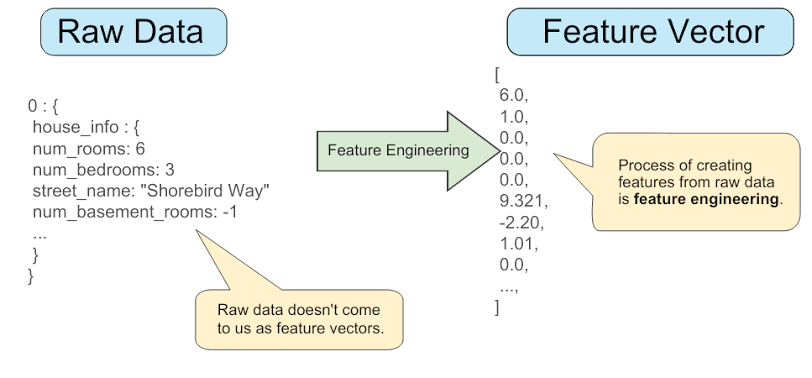
\includegraphics[scale=.5]{fe.png}}
\end{center}


\nd Complexity exists in the relationships between the input and output data. In the case of time series, there is no concept of input and output variables; we must invent these too and frame the supervised learning problem from scratch.

\nd A lag features is a fancy name for a variable which contains data from prior time steps. If we have time-series data, we can convert it into rows. Every row contains data about one observation and includes all previous occurrences of that observation.

\nd To generare Lag features the steps required are : 

\nd 1. Select only the time-series data related to that one observation.

\nd 2. Extract all values of the time-series variables

\nd 3. Shift the target variables five times to get five lag features and the new dependent feature 

\nd 4. Shift the other time-series variable six times to get all lag values of that independent feature.

\nd 5. Copy the non-time-series variables.

\nd 6. Split the data frame into the independent features and the dependent features.

\nd 7. Store them in arrays that will be used later for feature scaling, splitting into training/validation/test sets, and finally for the training of a model.

\newpage 
\subsection{\msize{\textbf{\textbf{RELU AND ADAM FUNCTIONS }}}}
The rectified linear is the activation function used in our code and adam function is the optimiser. 
\subsubsection{\textbf{RECTIFIED LINEAR FUNCTION}}
The Rectified Linear Function(RELU) goes as : 

\begin{equation*} 
\phi(z)=max(0,z)
\end{equation*}

\nd In a neural network, the activation function is responsible for transforming the summed weighted input from the node into the activation of the node or output for that input.

\nd The rectified linear activation function or ReLU for short is a piecewise linear function that will output the input directly if it is positive, otherwise, it will output zero. It has become the default activation function for many types of neural networks because a model that uses it is easier to train and often achieves better performance.

\nd In order to use stochastic gradient descent with backpropagation of errors to train deep neural networks, an activation function is needed that looks and acts like a linear function, but is, in fact, a nonlinear function allowing complex relationships in the data to be learned.

\nd A node or unit that implements this activation function is referred to as a rectified linear activation unit. Often, networks that use the rectifier function for the hidden layers are referred to as rectified networks.

\begin{center}
\centerline{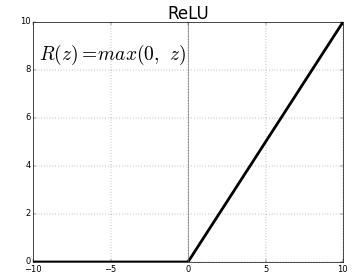
\includegraphics[scale=.7]{relu.png}}
\end{center}

\nd Because rectified linear units are nearly linear, they preserve many of the properties that make linear models easy to optimize with gradient-based methods. They also preserve many of the properties that make linear models generalize well.
\newpage
\subsubsection{\textbf{ADAM OPTIMIZER}}
The Adam optimization algorithm is an extension to stochastic gradient descent that has recently seen broader adoption for deep learning applications in computer vision and natural language processing.

\nd The choice of optimization algorithm for your deep learning model can mean the difference between good results in minutes, hours, and days

\nd Adam is an optimization algorithm that can be used instead of the classical stochastic gradient descent procedure to update network weights iterative based in training data.

\nd We have used adam because of : 

\nd 1. Straightforward to implement.

\nd 2.Computationally efficient.

\nd 3.Little memory requirements.

\nd 4.Invariant to diagonal rescale of the gradients.

\nd 5.Well suited for problems that are large in terms of data and/or parameters.

\nd 6.Appropriate for non-stationary objectives.

\nd 7.Appropriate for problems with very noisy/or sparse gradients.

\nd 8.Hyper-parameters have intuitive interpretation and typically require little tuning.

\nd Adam is different to classical stochastic gradient descent. Stochastic gradient descent maintains a single learning rate (termed alpha) for all weight updates and the learning rate does not change during training. A learning rate is maintained for each network weight (parameter) and separately adapted as learning unfolds. 

\nd The method computes individual adaptive learning rates for different parameters from estimates of first and second moments of the gradients.

\nd Adaptive Gradient Algorithm (AdaGrad) that maintains a per-parameter learning rate that improves performance on problems with sparse gradients (e.g. natural language and computer vision problems).

\nd Root Mean Square Propagation (RMSProp) that also maintains per-parameter learning rates that are adapted based on the average of recent magnitudes of the gradients for the weight (e.g. how quickly it is changing). This means the algorithm does well on online and non-stationary problems (e.g. noisy).

\nd For each parameter $w^j$

\begin{equation*}
\upsilon_t = \rho \, \upsilon_{t-1} + (1-\rho)* g^2_t
\end{equation*}

\begin{equation*}
\delta w_t= -\frac{\eta}{\sqrt{\upsilon_t + \epsilon}} * g_t
\end{equation*}

\begin{equation*}
w_{t+1}= w_{t-1} + \delta\,w_t
\end{equation*}

\nd Adam can be looked at as a combination of RMSprop and Stochastic Gradient Descent with momentum. It uses the squared gradients to scale the learning rate like RMSprop and it takes advantage of momentum by using moving average of the gradient instead of gradient itself like SGD with momentum.

\begin{center}
\centerline{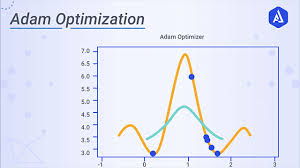
\includegraphics[scale=.7]{ada.png}}
\end{center}

\nd Adam is an adaptive learning rate method, which means, it computes individual learning rates for different parameters. Its name is derived from adaptive moment estimation, and the reason it’s called that is because Adam uses estimations of first and second moments of gradient to adapt the learning rate for each weight of the neural network. 

\newpage 
\section*{\mainsize{\textbf{REFERENCES}}}
\addcontentsline{toc}{section}{\protect\numberline{}\mainsize{\textbf{REFERENCES}}}
$[1]$ Fei-Yue Wang et al. Parallel control and management for intelligent transportation systems: Concepts, architectures, and applications. IEEE Transactions on Intelligent Transportation Systems, 2010.

\nd $[2]$ Yongchang Ma, Mashrur Chowdhury, Mansoureh Jeihani, and Ryan Fries. Accelerated incident detection across transportation networks using vehicle kinetics and support vector machine in cooperation with infrastructure agents. IET intelligent transport systems, 4(4):328–337, 2010.

\nd $[3]$ Rutger Claes, Tom Holvoet, and Danny Weyns. A decentralized approach for anticipatory vehicle routing using delegate multiagent systems. IEEE Transactions on Intelligent Transportation Systems, 12(2):364–373, 2011.

\nd $[4]$  Mehul Mahrishi and Sudha Morwal.Index point detection and semantic indexing of videos - a comparative review. Advances in Intelligent Systems and Computing, Springer, 2020.

\nd $[5]$ Joseph D Crabtree and Nikiforos Stamatiadis. Dedicated short-range communications technology for freeway incident detection: Performance assessment based on traffic simulation data. Transportation Research Record, 2000(1):59–69, 2007.

\nd $[6]$ H Qi, RL Cheu, and DH Lee. Freeway incident detection using kinematic data from probe vehicles. In 9th World Congress on Intel- ligent Transport SystemsITS America, ITS Japan, ERTICO (Intelligent Transport Systems and Services-Europe), 2002.

\nd $[7]$ Z. Zhao, W. Chen, X. Wu, P. C. Y. Chen, and J. Liu. Lstm network: a deep learning approach for short-term traffic forecast. IET Intelligent Transport Systems, 11(2):68–75, 2017.

\nd $[8]$ C. Zhang, P. Patras, and H. Haddadi. Deep learning in mobile and wireless networking: A survey. IEEE Communications Surveys Tutorials, 21(3):2224–2287, thirdquarter 2019.

\nd $[9]$ Chun-Hsin Wu, Jan-Ming Ho, and D. T. Lee. Travel-time prediction with support vector regression. IEEE Transactions on Intelligent Transportation Systems, 5(4):276–281, Dec 2004.

\nd $[10]$ Yan-Yan Song and LU Ying. Decision tree methods: applications for classification and prediction. Shanghai archives of psychiatry, 27(2):130, 2015.

\nd $[11]$ Yiming He, Mashrur Chowdhury, Yongchang Ma, and Pierluigi Pisu. Merging mobility and energy vision with hybrid electric vehicles and vehicle infrastructure integration. Energy Policy, 41:599–609, 2012.

\nd $[12]$ Jason Brownlee. Bagging and random forest ensemble algorithms for machine learning. Machine Learning Algorithms, pages 4–22, 2016.









\end{document}








